% !TeX root = ./00.ppgcc-2020.tex

\begin{fichacatalografica}
   %     \includepdf{fig_ficha_catalografica.pdf}
   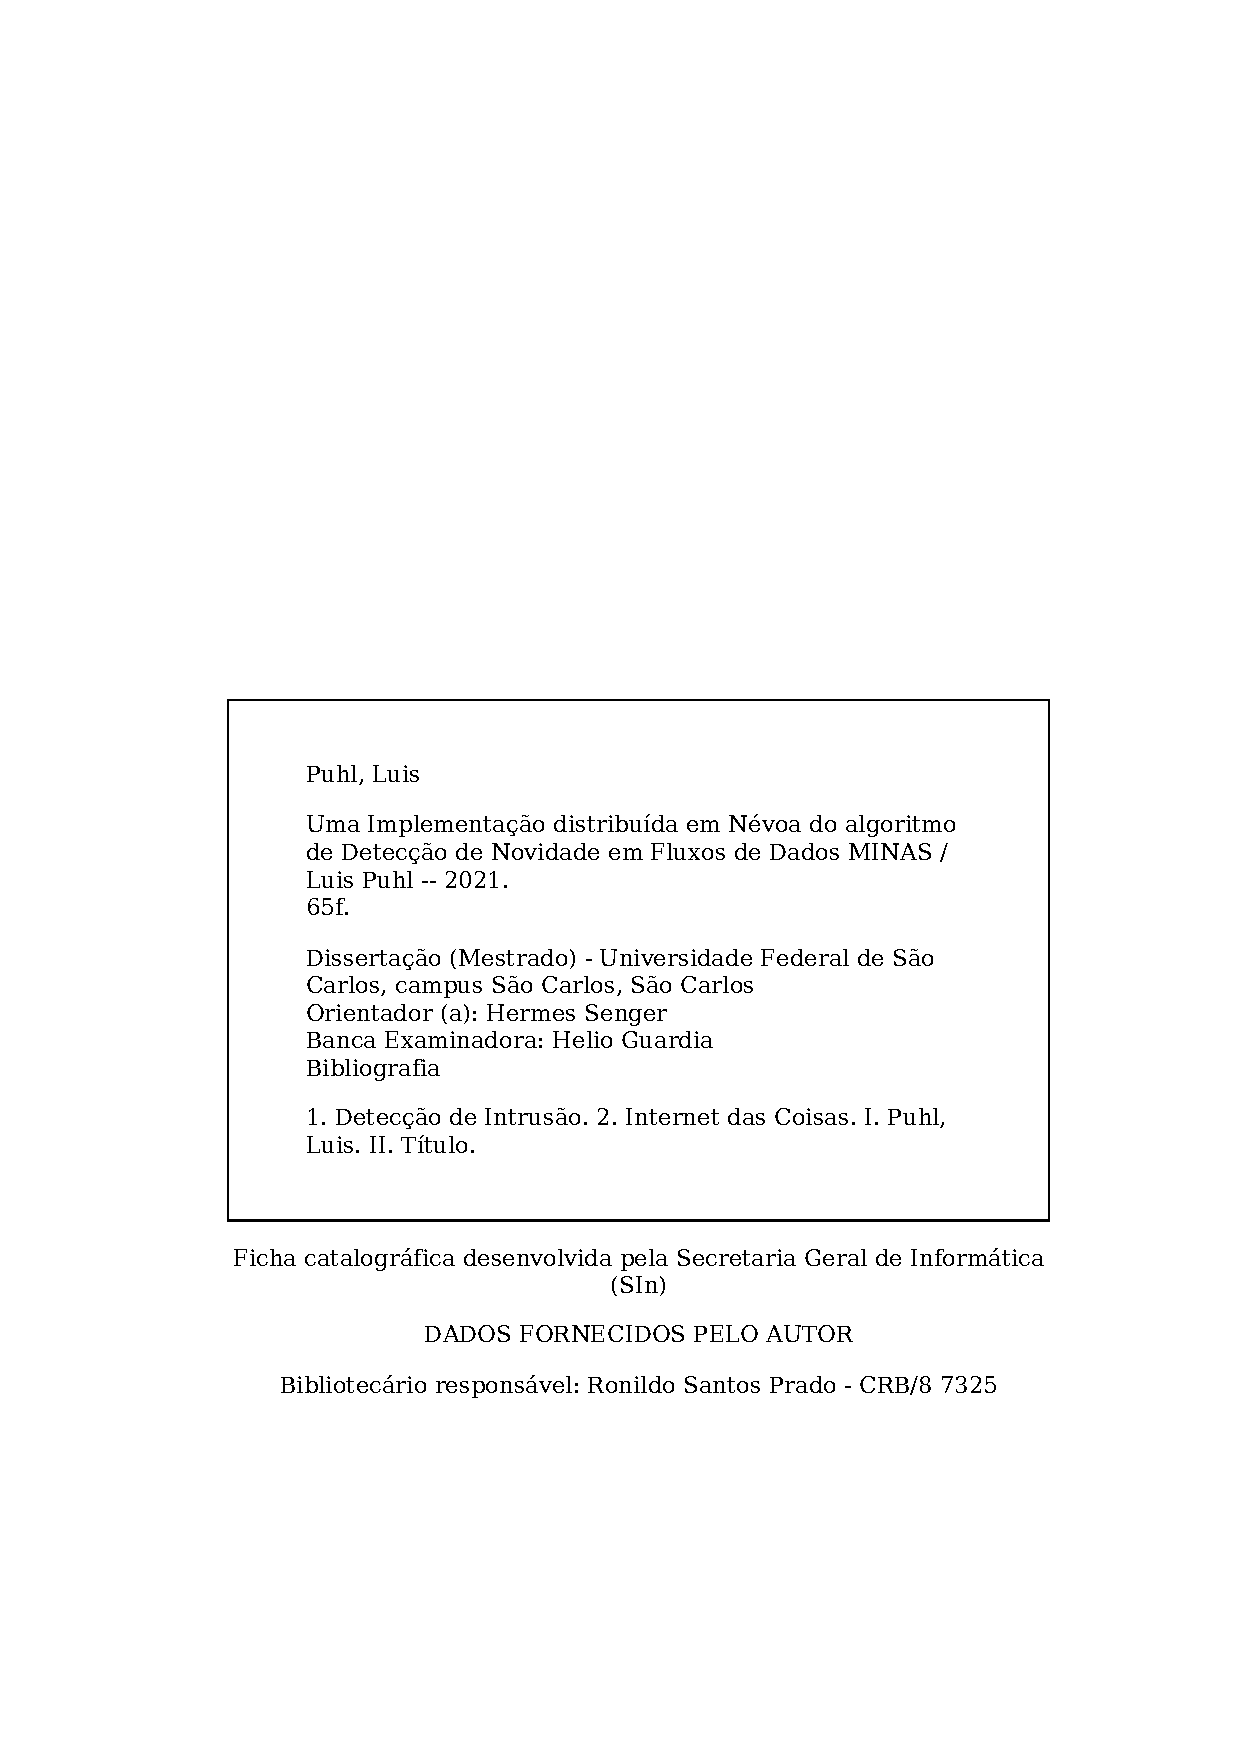
\includepdf{ficha-catalografica.pdf}
   % 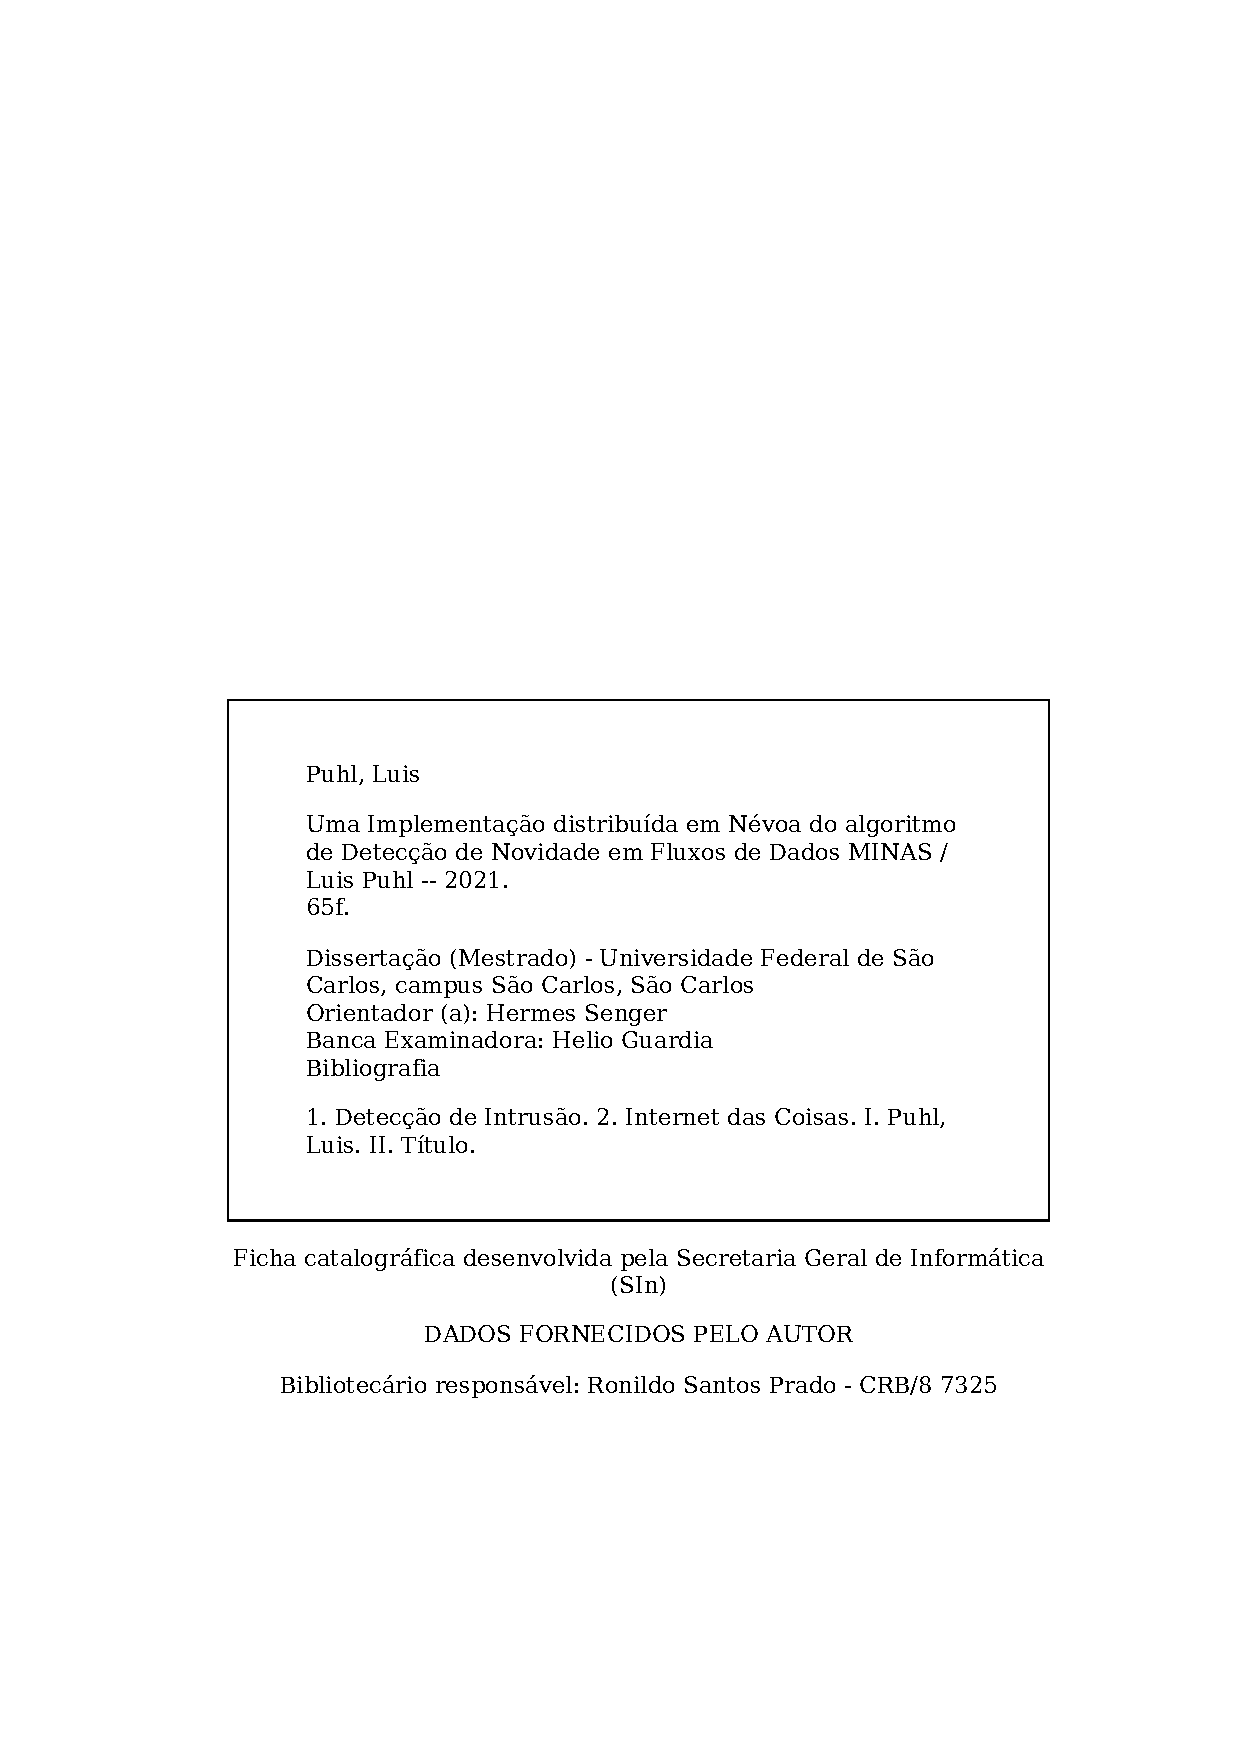
\includegraphics{ficha-catalografica.pdf}
   % \sffamily
   % \vspace*{\fill}                    % Posição vertical
   % \begin{center}                    % Minipage Centralizado
   %    \fbox{\begin{minipage}[c][8cm]{13.5cm}        % Largura
   %       \small
   %       % \imprimirautor
   %       % Puhl, Luís
   %       \authorbib
   %       %Sobrenome, Nome do autor
         
   %       \hspace{0.5cm} \imprimirtitulo  / \imprimirautor. --
   %       % \imprimirlocal, \imprimirdata-
         
   %       \hspace{0.5cm} \thelastpage{}f. : il. (algumas color.) ; 30 cm.\\
   %       % \pageref{LastPage}
         
   %       \hspace{0.5cm} \imprimirorientadorRotulo~\imprimirorientador\\
         
   %       \hspace{0.5cm}
   %       \parbox[t]{\textwidth}{\imprimirtipotrabalho~--~\@universidade
   %       % \imprimirinstituicao,
   %       \imprimirdata.}\\
         
   %       \hspace{0.5cm}
   %          1. Detecção de Intrusão.
   %          2. Internet das Coisas.
   %          I. Título.
   %          % I. Orientador.
   %          % II. Universidade Fede.
   %          % III. Faculdade de xxx.
   %          % IV. Título             
   %    \end{minipage}}
   % \end{center}
\end{fichacatalografica}

\begin{folhadeaprovacao}
   % \includepdf{folhadeaprovacao_final.pdf}
   %
   \noindent\begin{minipage}{0.3\textwidth}
      
\includegraphics[width=\linewidth]{lib/ufscar.pdf}
      \end{minipage}%
      \hfill%
      \begin{minipage}{0.7\textwidth}\center
      \imprimirinstituicao
   \end{minipage}
   % \begin{center}
   %    %   {\ABNTEXchapterfont\large\imprimirautor}

   %    %   \vspace*{\fill}\vspace*{\fill}
   %    %   \begin{center}
   %    %     \ABNTEXchapterfont\bfseries\Large\imprimirtitulo
   %    %   \end{center}
   %    %   \vspace*{\fill}

   %    %   \hspace{.45\textwidth}
   %    %   \begin{minipage}{.5\textwidth}
   %    %       \imprimirpreambulo
   %    %   \end{minipage}%
   %    %   \vspace*{\fill}
   % \end{center}
   
   \noindent\begin{minipage}{\textwidth}
      \begin{center}
      \rule{\linewidth}{1pt}
      % \vspace*{0.5ex}
      \textbf{Folha de Aprovação}\\[-0.5em]
      % \vspace*{-2ex}
      \rule{\linewidth}{1pt}
      % \hrule
      % \smash{\begin{tabular}{c} \hline  \\ \hline \end{tabular}\hspace*{-\tabcolsep}}
      % \frenchspacing
      % \hrulefill\\Folha de Aprovação\\\hrulefill
      \end{center}
   \end{minipage}

   % \vspace{2em}
   \begin{flushleft}
      Assinaturas dos membros da comissão examinadora que avaliou e aprovou a
      Defesa de Dissertação de Mestrado do candidato \imprimirautor{}, realizada
      em \today{}:
      %  Trabalho aprovado. \imprimirlocal, \today:
   \end{flushleft}
 
    \assinatura{\textbf{\imprimirorientador} \\ Orientador}
    \assinatura{\textbf{Professor} \\ Convidado 1}
    \assinatura{\textbf{Professor} \\ Convidado 2}
    %\assinatura{\textbf{Professor} \\ Convidado 3}
    %\assinatura{\textbf{Professor} \\ Convidado 4}
       
   \vspace*{\fill}
   \begin{center}
      \vspace*{0.5cm}
      {\large\imprimirlocal}
      \par
      {\large\imprimirdata}
      \vspace*{1cm}
   \end{center}
\end{folhadeaprovacao}

% Dedicatória
% \imprimirdedicatoria{Este trabalho é dedicado às crianças adultas que,\\
%    quando pequenas, sonharam em se tornar cientistas.}
% Agradecimentos
\imprimiragradecimentos{
   % Carolina, Guilherme Cassales, Guilherme Raiol, Jaime, Lucian, Pedro,
   
   Agradeço à constante compania, incentivo e ensinamentos dos colegas e
   agradeço especialmente à CNPq pelo suporte financiero (contrato 167345/2018-4).
}
% Epígrafe
% \imprimirepigrafe{
%         ``Somos essencialmente profissionais do sentido. Educamos, \\
%          quando ensinamos com sentido. Educar é impregnar de sentido\\
%          a vida. A profissão docente está centrada na vida, no bem querer.''\\
%         (Prof. Gilberto Teixeira)
% }

% RESUMO e ABSTRACT
\begin{resumo}{Detecção de Novidades. Detecção de Intrusão. Fluxos de Dados.
   Computação Distribuída. Computação em Névoa. Internet das Coisas}

   Em um cenário de crescente número de dispositivos na Internet das Coisas
   (IoT), gerando proporcional crescimento no volume dos fluxos de dados
   gerados, são necessários métodos robustos para a mineração de fluxos
   contínuos de dados.
   % 
   Uma das áreas afetadas pelo crescimento vertiginoso do número de dispositivos
   e os fluxos associados a eles é a área de segurança da informação, onde são
   necessárias ferramentas de detecção de intrusão em redes que operem em
   ambientes de computação em névoa, devido aos custos de comunicação associados
   a operar estas ferramentas somente em ambiente de nuvem.
   % 
   As ferramentas de detecção de intrusão utilizam extensivamente algoritmos de
   detecção de novidade em fluxos de dados para identificar padrões no tráfego
   da rede.
   % 
   Porém, os algoritmos que tratam adequadamente dos desafios de detecção de
   novidade em fluxos de dados, como mudança e evolução de conceito e
   atualização contínua do modelo de classificação sem interferência de
   especialistas, ainda são pouco utilizados.
   % 
   O algoritmo de detecção de novidade em fluxo de dados MINAS tem recebido
   atenção de pesquisas recentes por tratar desses desafios de detecção de
   novidade em fluxos de dados.
   % 
   No entanto, apesar de sua divisão em três partes semi-independentes, este
   algoritmo ainda não foi adaptado para processar grandes volumes de fluxos
   reais em ambiente de computação em névoa.
   % 
   O presente trabalho aborda essa lacuna, propondo um sistema
   que implementa o algoritmo MINAS de maneiraiot distribuída num contexto
   de detecção de intrusão e computação em névoa.
   % 
   Experimentos mostram que o algoritmo MINAS pode ser paralelizado e
   distribuído utilizando plataformas de processamento de fluxos como
   \emph{Apache Flink}.
\end{resumo}

% Resumo em inglês
\begin{abstract}{Novelty Detection. Intrusion Detection. Data Streams.
   Distributed Computing. Fog Computing. IoT devices}

   % In a scenario of growing number of devices connected to the Internet of Things (IoT)
   % with proportional growth in the volume of data streams generated, robust
   % methods are needed for mining streams continuous data.
   % %%
   % One of the areas affected by the huge growth in the number of devices
   % and the streams associated with them is the information security, which needs
   % network intrusion detection tools that operate
   % in fog computing environments due to the cost of operating such tools
   % in a cloud only environment.
   % %%
   % These tools make extensive use of algorithms for novelty detection in data
   % streams to identify treat patterns in network traffic.
   % However, algorithms in wide use do not
   % adequately address the challenges of novelty detection in data streams,
   % such as concept drift, concept evolution and continuous update of the
   % classification model, without expert interference.
   % %%
   % The MINAS algorithm addresses those novelty detection in data streams
   % challenges and has received recent research attention.
   % %%
   % However, despite its division in three semi-independent parts, MINAS has
   % not yet been adapted to process large volumes of real streams or to operate
   % in a fog computing environment.
   % %%
   % The present work proposes a system that implements the MINAS algorithm
   % in a distributed fog environment in the context of intrusion detection
   % to addresses this gap.
   % %%
   % Preliminary work shows that it is possible to have a distributed
   % version of the MINAS algorithm by using stream processing platforms
   % such as Apache Flink.

   The ongoing implementation of the Internet of Things (IoT) is sharply
   increasing the number and variety of small devices on edge networks.
   %
   Likewise, the attack opportunities for hostile agents also
   increases, requiring more effort from network administrators and strategies
   to detect and react to those threats.
   % 
   For a network security system to operate in the context of edge and
   IoT, it has to comply with processing, storage, and energy
   requirements alongside traditional requirements for stream and network
   analysis like accuracy and scalability.
   % 
   Using a previously defined architecture (IDSA-IoT), we address the construction
   and evaluation of a support mechanism for distributed Network Intrusion
   Detection Systems (NIDS) based on the MINAS Data Stream Novelty Detection
   % (DSND)
   algorithm.
   % 
   We discuss the algorithm steps, how it can be deployed in a distributed
   environment, the impacts on the accuracy and evaluate performance and
   scalability using a cluster of constrained devices commonly found in IoT
   scenarios.
   % 
   The obtained results show a negligible accuracy loss in the distributed
   version but also a small reduction in the execution time using low profile
   devices. Although not efficient, the parallel version showed to be viable as
   the proposed granularity provides equivalent accuracy and viable response times.

\end{abstract}
